\documentclass{article}

\usepackage{graphicx} % Required for inserting images
\usepackage{listings}
\usepackage{xcolor}

\lstset{
language=Python,
basicstyle=\ttfamily,
keywordstyle=\color{blue},
commentstyle=\color{green},
stringstyle=\color{red},
showstringspaces=false,
breaklines=true,
tabsize=4
}

\begin{document}
\begin{center}

\subsection{TRABALHO DE MATEMÁTICA}

MANUELA SILVA DE ANARDADE - 1º CICLO DE CIÊNCIA DE DADOS

\end{center}


1. Deduza A o determinante 4x4 usando a fórmula:

\begin{figure}[h]
    \centering
    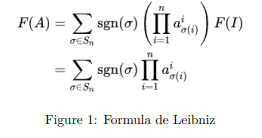
\includegraphics{Captura de tela 2023-05-09 075535.png}
    \label{fig:my_label}
\end{figure}

\begin{lstlisting}    
A = [a11 a12 a13 a14]
    [a21 a22 a23 a24]
    [a31 a32 a33 a34]
    [a41 a42 a43 a44]

det(A) =
a11*a22*a33*a44 + a11*a23*a34*a42 + a11*a24*a32*a43 + a12*a21*a34*a43
+ a12*a23*a31*a44 + a12*a24*a33*a41 + a13*a21*a32*a44 + a13*a22*a34*a41
+ a13*a24*a31*a42 + a14*a21*a33*a42 + a14*a22*a31*a43 + a14*a23*a32*a41
- a11*a22*a34*a43 - a11*a23*a32*a44 - a11*a24*a33*a42 - a12*a21*a33*a44
- a12*a23*a34*a41 - a12*a24*a31*a43 - a13*a21*a34*a42 - a13*a22*a31*a44
- a13*a24*a32*a41 - a14*a21*a32*a43 - a14*a22*a33*a41 - a14*a23*a31*a42

Exemplo:

A = [1 0 3 2]
    [2 1 1 0]
    [0 2 0 1]
    [-1 4 2 1]

det(A) = ( 1*1*0*1 + 1*1*1*4 + 1*0*2*2 + 0*2*1*2 + 0*1*0*1 + 0*0*0*(-1) + 3*2*2*1 + 3*1*1*(-1) + 3*0*0*4 + 2*2*0*4 + 2*1*0*2 + 2*1*2*(-1) - 1*1*1*2 - 1*1*2*1 - 1*0*0*4 - 0*2*0*1 - 0*1*1*(-1) - 0*0*0*2 - 3*2*1*4 - 3*1*0*1 - 3*0*2*(-1) - 2*2*2*2 -2*1*0*(-1) - 2*1*0*4)

det(A) = (0 + 4 + 0 + 0 + 0 + 0 + 12 + (-3) + 0 + 0 + 0 + 9 -(-4) - 2 - 2 - 0 - 0 - 0 - 0 - 24 - 0 - 0 - 16 - 0 - 0)

det(A) = (-35)

2. det(a) = 0 e det(a) != 0

A = [1 0 -1 2]
    [0 4 -2 0]
    [-1 0 1 2]
    [2 0 -2 4]
    
det(A) = 0

A = [1 0 2 0]
    [2 1 1 1]
    [2 3 0 1]
    [-1 1 2 2]
    
det(A) != 0  -> det(A) = 19

\end{lstlisting}

3. O código que replica a fórmula de Leibniz em python:

\begin{lstlisting}
    matriz = [[1, 0, -1, 2],
          [0, 4, -2, 0],
          [-1, 0, 1, 2],
          [2, 0, -2, 4]]

def leibniz(matriz):
    n = len(matriz)
    if n == 1:
        return matriz[0][0]
    else:
        soma = 0
        for j in range(n):
            nova_matriz = []
            for i in range(1, n):
                linha = []
                for k in range(n):
                    if k != j:
                        linha.append(matriz[i][k])
                nova_matriz.append(linha)
            sinal = (-1) ** j
            soma += matriz[0][j] * sinal * leibniz(nova_matriz)
        return soma

determinante = leibniz(matriz)

print("O determinante da matriz:", determinante)
\end{lstlisting}

\begin{figure}
    \centering
    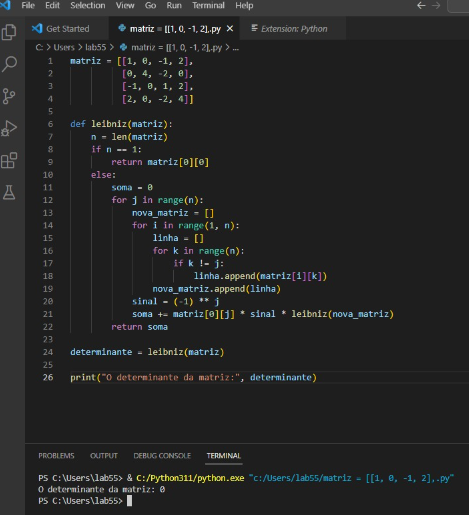
\includegraphics{fotocerta.png}
    \label{fig:my_label}
\end{figure}

\end{document}
